\subsection{Valve model}  
\label{ValveModel}

%R2015-1-S1 type valve

Valves in the water distribution system are modeled according to the assumption that the length of each valve, $L$, and the change in elevation, $\Delta z$, is zero. Therefore it is assumed that the length of the valve does not influence the flow and the pressure between the endpoints. The fact that the length of a valve is considerably smaller than the length of a pipe makes this a fair assumption. Another assumption is that in case of a valve, elevation is not present. 

In the given system, valves are considered as end-user components since they are placed only in the PMAs. These user valves have a variable Opening Degree(OD) which influences the pressure drop across the endpoints. 

%Valves can be also seen as pipe fittings where the OD is constant for all times, however there are not any fittings in the system, moreover the model of pipes covers it anyway. \\
%Due to the above-mentioned considerations, by recalling \eqref{FinalPipeModel}, it simplifies as follows: 
%
%\begin{equation}
%\label{ValveModel}
% \Delta p =  - k_f \frac{8q^2}{\pi^2gD^4} \rho g 
%\end{equation}

%In \eqref{ValveModel}, the form-loss coefficient is taken into account in order to determine the pressure drop. Although $k_f$ is a coefficient that describes the resistance of the valve,

In case of valves, manufacturers provide a parameter which indicates the valve capacity. This coefficient is called the $k_{v100}$- factor that describes the conductivity of the valve at maximum OD. This parameter sets the relationship between the water flow through the valve in $m^{3}$ in one hour. The experiments were carried out with a pressure drop of $\Delta p = 1 [bar]$ at a fully open state of the valve. According to \cite{kvvalve}, the properties of water fulfil the requirements which allows to write up the following expression for flow and pressure: 

\begin{equation}
\label{kvequation}
 q =  k_{v100} \sqrt{\Delta p} 
\end{equation}

\begin{minipage}[t]{0.20\textwidth}
Where\\
\hspace*{8mm} $k_{v100}$ 
\end{minipage}
\begin{minipage}[t]{0.68\textwidth}
\vspace*{2mm}
is the valve maximum capacity factor.
 \end{minipage}
\begin{minipage}[t]{0.10\textwidth}
\vspace*{2mm}
\textcolor{White}{te}$\unit{\frac{m^{3}}{h}}$
\end{minipage}

\eqref{kvequation} can be derived in detail using the law of continuity for each endpoint of the valve, however the exact derivations can be found in the datasheet \cite{kvvalve}. In the further description and derivations, the coefficients and all the technical considerations are based on this datasheet.  

\textbf{Valve conductivity function \texorpdfstring{$k_v(OD)$}{}}
\label{OD}

Instead of $k_{v100}$, more generally $k_v(OD)$ can be used which is a function of the opening degree, where $OD \in  [0,1]$. In case of user-operated valves, $k_{v}$ does not remain constant, it ranges over a compact set of values as the opening degree varies. \cite{Kallesoe2009}.

All valves in the system share the same characteristics, therefore the following characteristics of $k_{v}$ are valid for all of them. 

%k_v valve characteristics
%\begin{figure}[H]
%\label{valve_conductivity}
%\centering
%
\includegraphics[width=0.5\textwidth]{report/pictures/missingfigure}
%\caption{Valve characteristics - Valve conductivity in the function of OD}
%\end{figure}

\begin{figure}[H]
\centering
% This file was created by matlab2tikz.
%
%The latest updates can be retrieved from
%  http://www.mathworks.com/matlabcentral/fileexchange/22022-matlab2tikz-matlab2tikz
%where you can also make suggestions and rate matlab2tikz.
%
\definecolor{mycolor1}{rgb}{0.00000,0.44700,0.74100}%
%
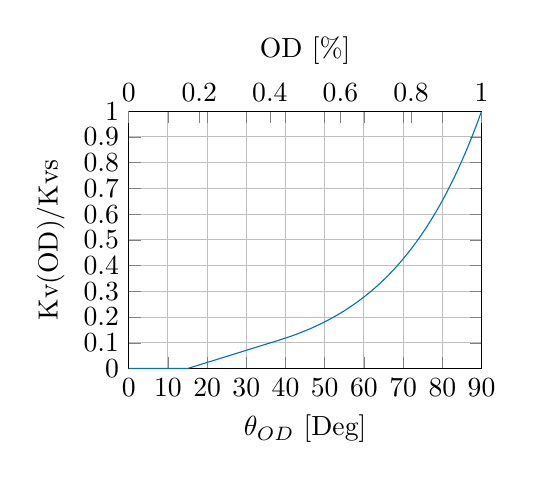
\begin{tikzpicture}

\begin{axis}[%
width=0.5\textwidth,
height=0.4\textwidth,
grid=both,
xmin=0,
xmax=90,
xtick = {0,10,20,30,40,50,60,70,80,90},
ytick = {0,0.1,0.2,0.3,0.4,0.5,0.6,0.7,0.8,0.9,1},
xlabel={$\theta_{OD}$ [Deg]},
ymin=0,
ymax=1,
ylabel={Kv(OD)/Kvs},
axis background/.style={fill=white}
]
\addplot [color=mycolor1,solid]
  table[row sep=crcr]{%
0	0\\
0.216	0\\
0.423	0\\
0.63	0\\
0.837	0\\
1.044	0\\
1.251	0\\
1.458	0\\
1.665	0\\
1.872	0\\
2.079	0\\
2.286	0\\
2.493	0\\
2.7	0\\
2.907	0\\
3.114	0\\
3.321	0\\
3.528	0\\
3.735	0\\
3.942	0\\
4.149	0\\
4.356	0\\
4.563	0\\
4.77	0\\
4.977	0\\
5.193	0\\
5.4	0\\
5.607	0\\
5.814	0\\
6.021	0\\
6.228	0\\
6.435	0\\
6.642	0\\
6.849	0\\
7.056	0\\
7.263	0\\
7.47	0\\
7.677	0\\
7.884	0\\
8.091	0\\
8.298	0\\
8.505	0\\
8.712	0\\
8.919	0\\
9.126	0\\
9.333	0\\
9.54	0\\
9.747	0\\
9.954	0\\
10.17	0\\
10.377	0\\
10.584	0\\
10.791	0\\
10.998	0\\
11.205	0\\
11.412	0\\
11.619	0\\
11.826	0\\
12.033	0\\
12.24	0\\
12.447	0\\
12.654	0\\
12.861	0\\
13.068	0\\
13.275	0\\
13.482	0\\
13.689	0\\
13.896	0\\
14.103	0\\
14.31	0\\
14.517	0\\
14.724	0\\
14.931	0\\
15.000	0.000694957409248559\\
15.354	0.0016735709039047\\
15.561	0.00265218439856082\\
15.768	0.00363079789321695\\
15.975	0.0046094113878731\\
16.182	0.00558802488252923\\
16.389	0.00656663837718535\\
16.596	0.00754525187184149\\
16.803	0.00852386536649762\\
17.01	0.00950247886115376\\
17.217	0.0104810923558099\\
17.424	0.011459705850466\\
17.631	0.0124383193451222\\
17.838	0.0134169328397783\\
18.045	0.0143955463344344\\
18.252	0.0153741598290906\\
18.459	0.0163527733237467\\
18.666	0.0173313868184028\\
18.873	0.018310000313059\\
19.08	0.0192886138077151\\
19.287	0.0202672273023712\\
19.494	0.0212458407970273\\
19.701	0.0222244542916835\\
19.908	0.0232030677863396\\
20.124	0.0242242296938069\\
20.331	0.025202843188463\\
20.538	0.0261814566831191\\
20.745	0.0271600701777753\\
20.952	0.0281386836724314\\
21.159	0.0291172971670875\\
21.366	0.0300959106617437\\
21.573	0.0310745241563998\\
21.78	0.032053137651056\\
21.987	0.0330317511457121\\
22.194	0.0340103646403682\\
22.401	0.0349889781350244\\
22.608	0.0359675916296805\\
22.815	0.0369462051243366\\
23.022	0.0379248186189928\\
23.229	0.0389034321136489\\
23.436	0.039882045608305\\
23.643	0.0408606591029611\\
23.85	0.0418392725976173\\
24.057	0.0428178860922734\\
24.264	0.0437964995869295\\
24.471	0.0447751130815857\\
24.678	0.0457537265762418\\
24.885	0.046732340070898\\
25.101	0.0477535019783652\\
25.308	0.0487321154730213\\
25.515	0.0497107289676775\\
25.722	0.0506893424623336\\
25.929	0.0516679559569897\\
26.136	0.0526465694516459\\
26.343	0.053625182946302\\
26.55	0.0546037964409581\\
26.757	0.0555824099356143\\
26.964	0.0565610234302704\\
27.171	0.0575396369249265\\
27.378	0.0585182504195827\\
27.585	0.0594968639142388\\
27.792	0.0604754774088949\\
27.999	0.061454090903551\\
28.206	0.0624327043982072\\
28.413	0.0634113178928633\\
28.62	0.0643899313875195\\
28.827	0.0653685448821756\\
29.034	0.0663471583768317\\
29.241	0.0673257718714879\\
29.448	0.068304385366144\\
29.655	0.0692829988608001\\
29.862	0.0702616123554563\\
30.078	0.0712827742629235\\
30.285	0.0722613877575797\\
30.492	0.0732400012522358\\
30.699	0.0742186147468919\\
30.906	0.0751972282415481\\
31.113	0.0761758417362042\\
31.32	0.0771544552308603\\
31.527	0.0781330687255165\\
31.734	0.0791116822201726\\
31.941	0.0800902957148287\\
32.148	0.0810689092094849\\
32.355	0.082047522704141\\
32.562	0.0830261361987971\\
32.769	0.0840047496934533\\
32.976	0.0849833631881094\\
33.183	0.0859619766827655\\
33.39	0.0869405901774216\\
33.597	0.0879192036720778\\
33.804	0.0888978171667339\\
34.011	0.0898764306613901\\
34.218	0.0908550441560462\\
34.425	0.0918336576507023\\
34.632	0.0928122711453585\\
34.839	0.0937908846400146\\
35.055	0.0948120465474818\\
35.262	0.095790660042138\\
35.469	0.0967692735367941\\
35.676	0.0977478870314503\\
35.883	0.0987265005261064\\
36.09	0.0997051140207625\\
36.297	0.100683727515419\\
36.504	0.101662341010075\\
36.711	0.102640954504731\\
36.918	0.103619567999387\\
37.125	0.104598181494043\\
37.332	0.105576794988699\\
37.539	0.106555408483355\\
37.746	0.107534021978012\\
37.953	0.108512635472668\\
38.16	0.109491248967324\\
38.367	0.11046986246198\\
38.574	0.111450358774874\\
38.781	0.112439047968232\\
38.988	0.113436507939287\\
39.195	0.114442816494636\\
39.402	0.115458052131107\\
39.609	0.116482294041882\\
39.816	0.117515622122678\\
40.032	0.118603652037063\\
40.239	0.119655798933231\\
40.446	0.120717279547815\\
40.653	0.121788176681324\\
40.86	0.1228685738688\\
41.067	0.123958555386336\\
41.274	0.125058206257648\\
41.481	0.126167612260705\\
41.688	0.127286859934424\\
41.895	0.128416036585419\\
42.102	0.129555230294812\\
42.309	0.130704529925101\\
42.516	0.131864025127094\\
42.723	0.133033806346903\\
42.93	0.134213964832998\\
43.137	0.135404592643324\\
43.344	0.136605782652482\\
43.551	0.137817628558978\\
43.758	0.139040224892523\\
43.965	0.140273667021418\\
44.172	0.141518051159982\\
44.379	0.142773474376067\\
44.586	0.144040034598623\\
44.793	0.145317830625339\\
45	0.14660696213035\\
45.216	0.14796433706973\\
45.423	0.149276946043549\\
45.63	0.150601199325397\\
45.837	0.151937200213295\\
46.044	0.153285052921633\\
46.251	0.154644862589299\\
46.458	0.156016735287881\\
46.665	0.157400778029939\\
46.872	0.158797098777356\\
47.079	0.160205806449755\\
47.286	0.161627010933\\
47.493	0.163060823087764\\
47.7	0.164507354758179\\
47.907	0.165966718780558\\
48.114	0.167439028992201\\
48.321	0.168924400240268\\
48.528	0.170422948390744\\
48.735	0.171934790337476\\
48.942	0.173460044011288\\
49.149	0.174998828389181\\
49.356	0.176551263503618\\
49.563	0.178117470451882\\
49.77	0.179697571405526\\
49.977	0.181291689619898\\
50.193	0.182970196510922\\
50.4	0.184593346566117\\
50.607	0.186230895775666\\
50.814	0.187882971876154\\
51.021	0.189549703737333\\
51.228	0.191231221372175\\
51.435	0.192927655947008\\
51.642	0.194639139791758\\
51.849	0.19636580641026\\
52.056	0.198107790490679\\
52.263	0.199865227916016\\
52.47	0.201638255774704\\
52.677	0.203427012371305\\
52.884	0.205231637237295\\
53.091	0.207052271141952\\
53.298	0.208889056103334\\
53.505	0.210742135399357\\
53.712	0.212611653578975\\
53.919	0.21449775647345\\
54.126	0.216400591207731\\
54.333	0.218320306211929\\
54.54	0.220257051232897\\
54.747	0.22221097734591\\
54.954	0.224182236966449\\
55.17	0.226257850197162\\
55.377	0.228265010101009\\
55.584	0.230289975755579\\
55.791	0.232332905117774\\
55.998	0.234393957545747\\
56.205	0.23647329381134\\
56.412	0.238571076112618\\
56.619	0.240687468086527\\
56.826	0.242822634821652\\
57.033	0.244976742871101\\
57.24	0.247149960265492\\
57.447	0.249342456526065\\
57.654	0.2515544026779\\
57.861	0.253785971263261\\
58.068	0.256037336355057\\
58.275	0.258308673570416\\
58.482	0.260600160084386\\
58.689	0.262911974643757\\
58.896	0.265244297581001\\
59.103	0.267597310828342\\
59.31	0.269971197931946\\
59.517	0.272366144066237\\
59.724	0.274782336048345\\
59.931	0.277219962352675\\
60.147	0.279786630566282\\
60.354	0.282268650553725\\
60.561	0.28477268883134\\
60.768	0.28729894072596\\
60.975	0.289847603297184\\
61.182	0.29241887535275\\
61.389	0.295012957464044\\
61.596	0.297630051981744\\
61.803	0.300270363051602\\
62.01	0.302934096630374\\
62.217	0.305621460501882\\
62.424	0.308332664293221\\
62.631	0.311067919491114\\
62.838	0.313827439458407\\
63.045	0.316611439450714\\
63.252	0.319420136633203\\
63.459	0.322253750097546\\
63.666	0.325112500878996\\
63.873	0.32799661197364\\
64.08	0.330906308355789\\
64.287	0.333841816995525\\
64.494	0.336803366876412\\
64.701	0.339791189013351\\
64.908	0.342805516470604\\
65.124	0.345979414970217\\
65.331	0.349048638905121\\
65.538	0.352145090285227\\
65.745	0.355269010648395\\
65.952	0.35842064367519\\
66.159	0.361600235207901\\
66.366	0.364808033269708\\
66.573	0.368044288084039\\
66.78	0.371309252094077\\
66.987	0.374603179982464\\
67.194	0.377926328691159\\
67.401	0.381278957441482\\
67.608	0.384661327754338\\
67.815	0.388073703470612\\
68.022	0.391516350771757\\
68.229	0.394989538200547\\
68.436	0.398493536682034\\
68.643	0.402028619544678\\
68.85	0.405595062541667\\
69.057	0.409193143872427\\
69.264	0.412823144204324\\
69.471	0.41648534669456\\
69.678	0.420180037012252\\
69.885	0.423907503360728\\
70.101	0.427832292561157\\
70.308	0.431627642965361\\
70.515	0.43545666236777\\
70.722	0.439319649450014\\
70.929	0.443216905543361\\
71.136	0.447148734652225\\
71.343	0.451115443477877\\
71.55	0.455117341442374\\
71.757	0.459154740712688\\
71.964	0.463227956225065\\
72.171	0.467337305709585\\
72.378	0.47148310971495\\
72.585	0.475665691633485\\
72.792	0.479885377726369\\
72.999	0.48414249714908\\
73.206	0.488437381977074\\
73.413	0.492770367231687\\
73.62	0.497141790906269\\
73.827	0.501551993992547\\
74.034	0.506001320507227\\
74.241	0.510490117518827\\
74.448	0.515018735174751\\
74.655	0.519587526728602\\
74.862	0.524196848567735\\
75.078	0.529050176508021\\
75.285	0.533743442622258\\
75.492	0.538478343250191\\
75.699	0.543255247736467\\
75.906	0.548074528702238\\
76.113	0.55293656207422\\
76.32	0.557841727114017\\
76.527	0.56279040644771\\
76.734	0.567782986095699\\
76.941	0.572819855502817\\
77.148	0.577901407568706\\
77.355	0.58302803867847\\
77.562	0.58820014873359\\
77.769	0.593418141183118\\
77.976	0.598682423055154\\
78.183	0.603993404988588\\
78.39	0.609351501265138\\
78.597	0.614757129841662\\
78.804	0.620210712382765\\
79.011	0.625712674293686\\
79.218	0.631263444753484\\
79.425	0.636863456748515\\
79.632	0.642513147106209\\
79.839	0.648212956529143\\
80.055	0.654214499769577\\
80.262	0.660018113263248\\
80.469	0.665873211292337\\
80.676	0.67178025058219\\
80.883	0.677739691909819\\
81.09	0.683752000139841\\
81.297	0.689817644260743\\
81.504	0.695937097421464\\
81.711	0.702110836968301\\
81.918	0.708339344482148\\
82.125	0.714623105816057\\
82.332	0.720962611133143\\
82.539	0.727358354944811\\
82.746	0.733810836149338\\
82.953	0.740320558070785\\
83.16	0.74688802849826\\
83.367	0.753513759725527\\
83.574	0.760198268590969\\
83.781	0.766942076517901\\
83.988	0.773745709555248\\
84.195	0.780609698418574\\
84.402	0.787534578531486\\
84.609	0.794520890067394\\
84.816	0.80156917799165\\
85.032	0.808990584851016\\
85.239	0.816167235133375\\
85.446	0.823407550321407\\
85.653	0.830712095193952\\
85.86	0.838081439540067\\
86.067	0.845516158203477\\
86.274	0.853016831127412\\
86.481	0.860584043399844\\
86.688	0.868218385299134\\
86.895	0.875920452340067\\
87.102	0.883690845320312\\
87.309	0.891530170367282\\
87.516	0.89943903898542\\
87.723	0.907418068103896\\
87.93	0.91546788012473\\
88.137	0.923589102971344\\
88.344	0.931782370137542\\
88.551	0.940048320736924\\
88.758	0.948387599552746\\
88.965	0.956800857088209\\
89.172	0.965288749617202\\
89.379	0.973851939235501\\
89.586	0.982491093912409\\
89.793	0.991206887542863\\
90	1\\
};
\end{axis}

\begin{axis}[
  width=0.5\textwidth,
  height=0.4\textwidth,
  axis x line*=top,
  axis y line=none,
  %x filter/.code={\pgfmathparse{#1*1,111111111111111}\pgfmathresult},
  xmin=0,  
  xmax=100,
  xtick = {0,10,20,30,40,50,60,70,80,90,100},
  xlabel={OD [\%]}
]

\end{axis}
\end{tikzpicture}% 
\caption{Valve characteristics - Valve conductivity in the function of OD.}
\label{valve_conductivity}
\end{figure}

According to \cite{keller}, the following definition can be written up generally for the conductivity function, $k_v(OD)$:


\begin{equation}
\label{kvFunction}
 k_v(OD) =
		\left\{
		\begin{array}{ll}
		
		k_{v100} \, \frac{\theta_{OD}}{\theta_{max}} \, n_{gl} \, e^{(1-n_{gl})} \text{,} & \mbox{ if } 								\frac{\theta_{OD}}{\theta_{max}} \leq \frac{1}					{n_{gl}} \text{;}
\\
		k_{v100} \, e^{(n_{gl} \,(\frac{\theta_{OD}}{\theta_{max}}-1))} \text{,} & \mbox{ if } \frac{\theta_{OD}}{\theta_{max}} \geq \frac{1}{n_{gl}}

		\end{array}
		\right.
\end{equation}	

 \begin{minipage}[t]{0.20\textwidth}
Where\\
\hspace*{8mm} $\theta_{OD}$ \\
\hspace*{8mm} $\theta_{max}$ \\
%\hspace*{8mm}  \\
and \hspace*{0.7mm} $n_{gl}$ 
\end{minipage}
\begin{minipage}[t]{0.68\textwidth}
\vspace*{2mm}
is the opening degree,\\ 
is the upper opening degree, \\
is the valve characteristic curve factor.
\end{minipage}
\begin{minipage}[t]{0.10\textwidth}
\vspace*{2mm}
\textcolor{White}{te}$\unit{\degree}$\\
\textcolor{White}{te}$\unit{\degree}$\\
%\textcolor{White}{te}\\
\textcolor{White}{te}$\unit{\cdot}$
\end{minipage}	

A new parameter, $\theta_{max}$, is introduced which describes the maximum angle where the actuator closes the valve. The same can be stated for a minimum angle. The valve is closed when the position of the actuator $\in [0\degree,15\degree]$. As a consequence, there is an offset in the curve as it is shown in \figref{valve_conductivity}. Introducing the following angle:

\begin{equation}
\label{ValveAngle}
 \gamma =  \frac{\theta_{OD}-\theta_{off}}{\theta_{max}-\theta_{off}}
\end{equation}

  \begin{minipage}[t]{0.20\textwidth}
Where\\
\hspace*{8mm} $\theta_{off}$  
\end{minipage}
\begin{minipage}[t]{0.68\textwidth}
\vspace*{2mm}
is the minimum angle where the valve opens.

\end{minipage}
\begin{minipage}[t]{0.10\textwidth}
\vspace*{2mm}
\textcolor{White}{te}$\unit{\degree}$
\end{minipage}

In case of the water distribution system \eqref{kvFunction} modifies to: 

\begin{equation}
 k_v(OD) =
		\left\{
		\begin{array}{ll}
		
		k_{v100} \, \gamma \, n_{gl} \, e^{(1-n_{gl})} \text{,} & \mbox{ if } 	\gamma \leq \frac{1}					{n_{gl}} \text{;}
\\
		k_{v100} \, e^{(n_{gl} \,\gamma)} \text{,} & \mbox{ if } \gamma \geq \frac{1}{n_{gl}}

		\end{array}
		\right.
\end{equation}	

As it is shown, the conductivity function of the valve consists of two types of functions: 

\begin{equation}
 k_v(OD) =
		\left\{
		\begin{array}{ll}
		
		k_v(\theta_{OD}) \sim linear() \text{,} & \mbox{ if } 	\gamma \leq \frac{1}					{n_{gl}} \text{;}
\\
		k_v(\theta_{OD}) \sim exponential() \text{,} & \mbox{ if } \gamma \geq \frac{1}{n_{gl}}

		\end{array}
		\right.
\end{equation}	

Since exponential functions never cross the zero point, it is reasonable to use linear characteristics in the lower range. The transition from linear to exponential has to be continuously differentiable and predetermined by $n_{gl}$ \citep{Kallesoe2009,keller} 


\textbf{Complete valve model}
\label{unittransform}

Using \eqref{kvequation} with the conductivity function $k_v(OD)$ and expressing $\Delta p$ yields: 

\begin{equation}
\label{CompleteValveModel}
 \Delta p = \frac{1}{k_v(OD)^2} |q| q
\end{equation}

Describing it in a compact form for the $k^{th}$ valve in the network yields: 

\begin{equation}
\label{CompactValveModel}
 \Delta p_k = \mu_k(q_k,k_v(OD)) 
\end{equation}





 
 
 